I presenter sono organizzati specularmente alle viste ed espongono le funzionalità necessarie per le pagine che gestiscono e definiscono la logica di controllo prelevando le informazioni dal modello. La classe base espone un metodo \texttt{update} che, usando Express, provoca l'aggiornamento della vista. Per offrire le funzionalità alle viste, i presenter hanno un riferimento alla vista e uno al modello dei dati.
\begin{itemize}
	\item \texttt{DeveloperPresenter}: il presenter dedicato alle funzionalità dello sviluppatore che necessita di consultare i dati ed il loro storico;
	\item \texttt{ProfilePresenter}: il presenter che si occupa di recuperare le informazioni legate a un singolo utente (ad esempio, la media degli esercizi per lo studente o il numero di esercizi assegnati per l'insegnante)
	\item \texttt{SearchPresenter}: il presenter dedicato alle funzionalità di ricerca nella piattaforma, come quella degli utenti e degli esercizi;
	\item \texttt{ExercisePresenter}: il presenter dedicato allo svolgimento e all'inserimento di un esercizio nella piattaforma.
\end{itemize}

\begin{figure}[h]
	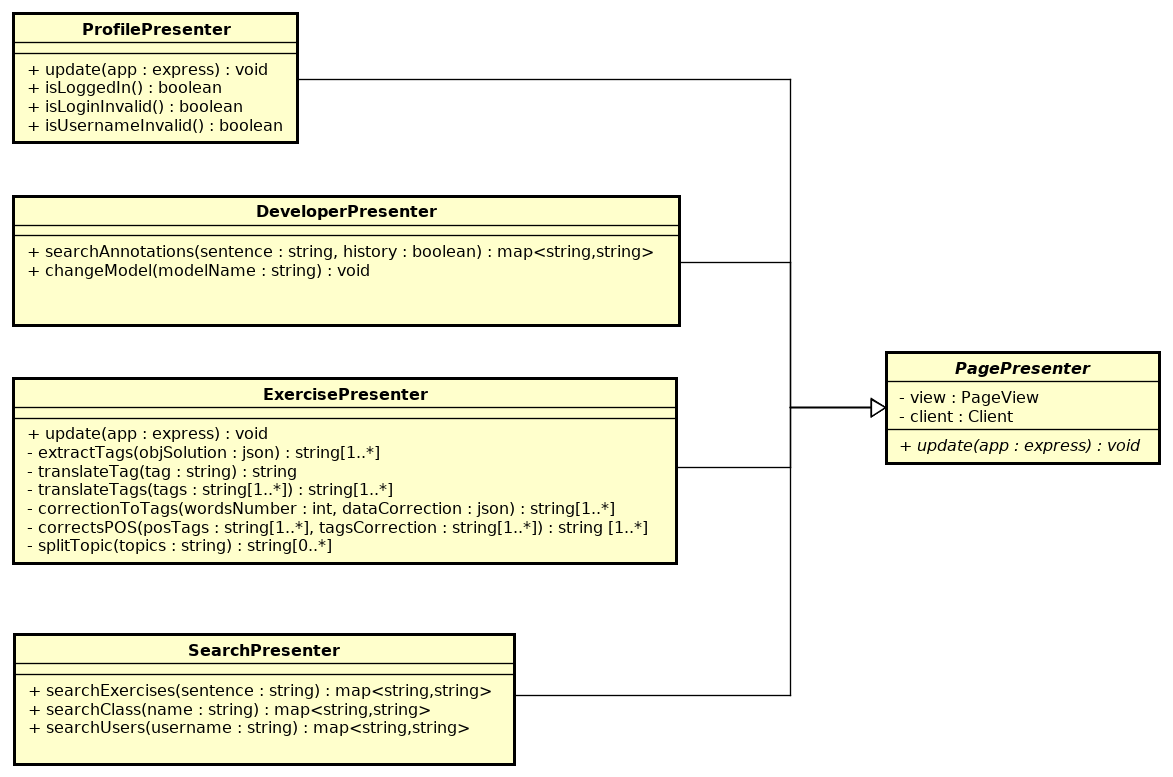
\includegraphics[scale=0.53]{images/Presenter.png}
	\caption{Diagramma delle classi del package Presenter}
\end{figure}
